\documentclass[12pt]{amsart}
%\pagestyle{empty} 
\setlength{\topmargin}{-0.4in} % usually -0.25in
\addtolength{\textheight}{1.45in} % usually 1.25in
\addtolength{\oddsidemargin}{-0.8in}
\addtolength{\evensidemargin}{-0.8in}
\addtolength{\textwidth}{1.5in} %\setlength{\parindent}{0pt}

% macros
\usepackage{wrapfig,caption,palatino,tabularx}
\usepackage{amssymb,xspace}
\usepackage[final]{graphicx}
\usepackage[colorlinks=true]{hyperref}

\newtheorem*{lem*}{Lemma}

\newcommand{\mtt}{\texttt}
\newcommand{\mtl}[1]{{\texttt{>>#1}}}

\newcommand{\CC}{{\mathbb{C}}}
\newcommand{\RR}{{\mathbb{R}}}
\newcommand{\eps}{\epsilon}
\newcommand{\ZZ}{{\mathbb{Z}}}
\newcommand{\ZZn}{{\mathbb{Z}}_n}
\newcommand{\NN}{{\mathbb{N}}}
\newcommand{\bu}{\mathbf{u}}
\newcommand{\bv}{\mathbf{v}}
\newcommand{\ip}[2]{\mathrm{\left<#1,#2\right>}}
\newcommand{\erf}{\operatorname{erf}}
\newcommand{\spn}{\operatorname{span}}

\newcommand{\prob}[1]{\bigskip\bigskip\noindent\large\textbf{#1.} \normalsize}
\newcommand{\bookprob}[1]{\bigskip\bigskip\noindent\large\textbf{Exercise #1.} \normalsize}
\newcommand{\ppart}[1]{\medskip\noindent\large\textbf{\emph{#1})}\normalsize}

\newcommand{\textbook}{\textsc{Trefethen \& Bau}}

\begin{document}

\begin{center}
\Huge Math 617 Functional Analysis

\Large \medskip

Spring 2024, UAF
\end{center}

\thispagestyle{empty}
\vspace{12mm}

\noindent \emph{instructor:} \begin{minipage}[t]{0.5\textwidth} Ed Bueler \\ \texttt{elbueler\@@alaska.edu} \end{minipage} \hfill \emph{CRN:}\, \begin{minipage}[t]{0.25\textwidth} 35367 (in-person) \\ 35378 (sync zoom) \end{minipage}

\medskip
\noindent \emph{course website:} \href{https://bueler.github.io/fa/}{\texttt{bueler.github.io/fa/}} \hfill \emph{room \& time:} \begin{minipage}[t]{0.25\textwidth} Chapman 107 \\ MWF 2:15--3:15 pm \end{minipage}

\medskip
\noindent \emph{textbook:} \begin{minipage}[t]{0.55\textwidth} D. Borthwick, \emph{Spectral Theory: Basic Concepts and Applications}, Springer 2020 \end{minipage}

\bigskip
\noindent \emph{prerequisites:} \begin{minipage}[t]{0.52\textwidth} linear algebra, undergrad/grad real analysis, exposure to complex analysis \end{minipage}

\vspace{-20mm}
\hfill 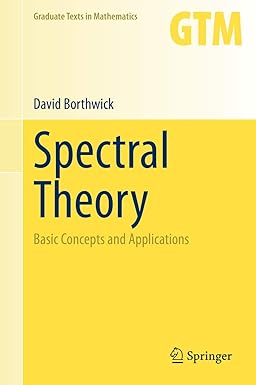
\includegraphics[height=45mm]{../../images/borthwick.jpg}

\vspace{4mm}

\begin{minipage}[t]{0.35\textwidth}
\smallskip

\centering
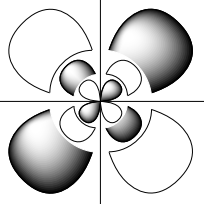
\includegraphics[width=\textwidth]{../../images/boundstates.png}
\end{minipage}
\hfill
\begin{minipage}[t]{0.55\textwidth} \vspace{0mm} Functional analysis is about infinite-dimensional vector spaces---spaces of functions---and their linear maps.  It is the mathematical home of partial differential equations, boundary value problems, quantum mechanics, the finite element method, field theories, fluid mechanics, and signal processing.

\medskip
\noindent This course should appeal to students interested in the mathematics of quantum mechanics and/or partial differential equations.  Mathematically-inclined students from the sciences and engineering are encouraged to attend, as are graduate students in mathematics looking for an elective with practical relevance.
\end{minipage}

\bigskip
\noindent While the course is delivered hybrid, in-person attendance is recommended!

\bigskip \noindent 
\begin{minipage}[t]{0.55\textwidth} \emph{Topics:}
\begin{itemize}
\item Hilbert spaces
\item Riesz representation theorems
\item Sobolev spaces (light)
\item self-adjoint operators: compact, bounded
\item unbounded operators
\item spectral theorem
\item Laplacians and Hamiltonians
\item axioms/concepts of quantum mechanics
\end{itemize}
\end{minipage}
\hfill
\begin{minipage}[t]{0.4\textwidth}
\smallskip

\centering
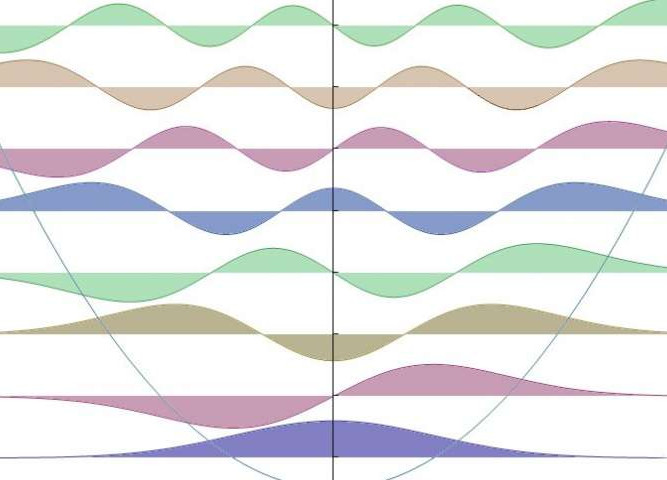
\includegraphics[width=\textwidth]{../../images/harmonic.jpg}
\end{minipage}

\end{document}
